\subsubsection{Infinite Horizon}
\begin{frame}{\subsecname: \subsubsecname}
    \begin{figure}
        \centering
        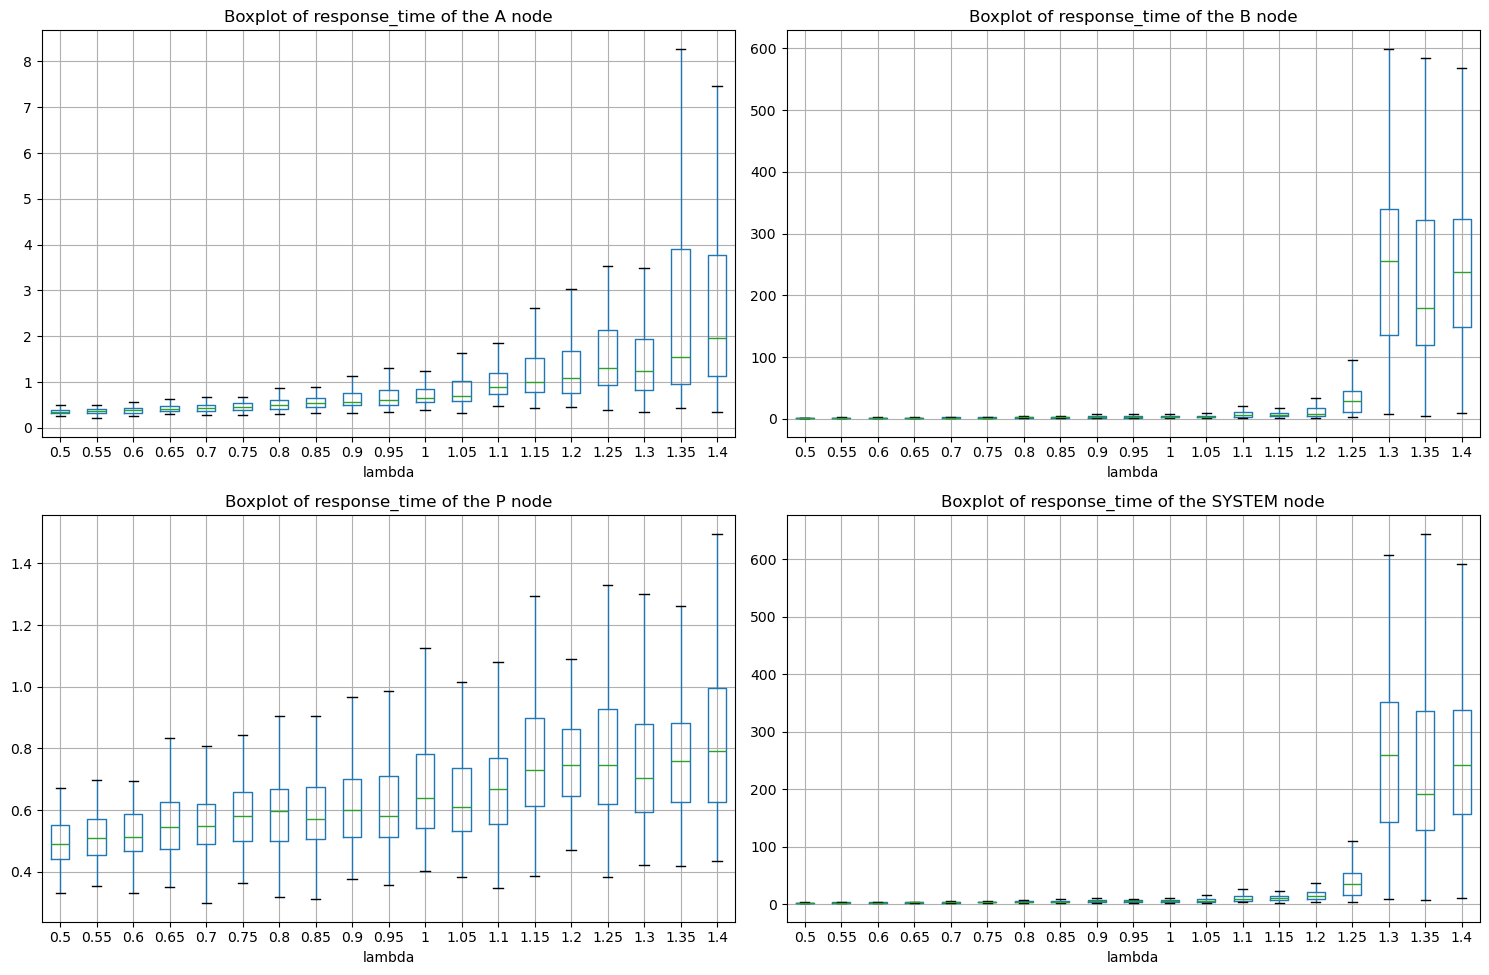
\includegraphics[width=0.75\linewidth]{figs/results/obj3/simulation/obj3_boxplot_rtime.png}
        \caption{Distribuzione del Tempo di Risposta medio dei risultati sperimentali dell’obbiettivo 3}
        \label{fig:enter-label}
    \end{figure}
\end{frame}

\subsubsection{Finite Horizon}
\begin{frame}{\subsecname: \subsubsecname}
    \begin{figure}
        \centering
        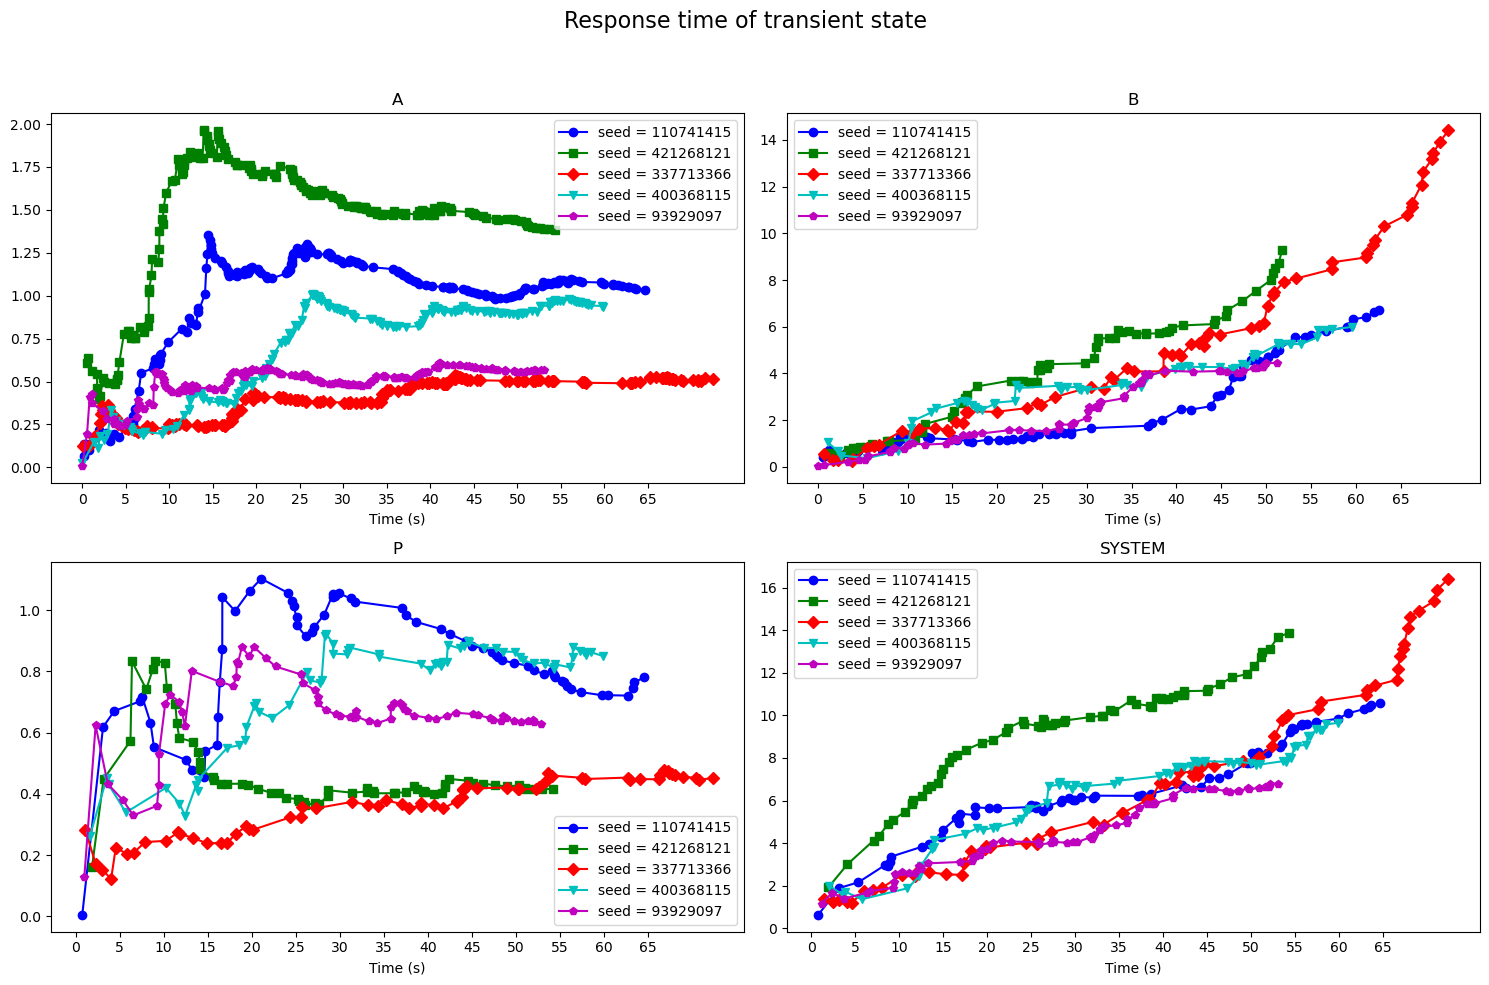
\includegraphics[width=0.75\linewidth]{figs/appendices/transient/obj3-transient-rtime-analitycal.png}
        \caption{Tempo di risposta per l’obiettivo 3 in funzione del tempo di simulazione nello stato transiente del sistema con un rate di arrivi 1.4 $job/s$ al variare del seed}
        \label{fig:enter-label}
    \end{figure}
\end{frame}

\subsubsection{Verification}
\begin{frame}{\subsecname: \subsubsecname}
\begin{figure}
    \centering
    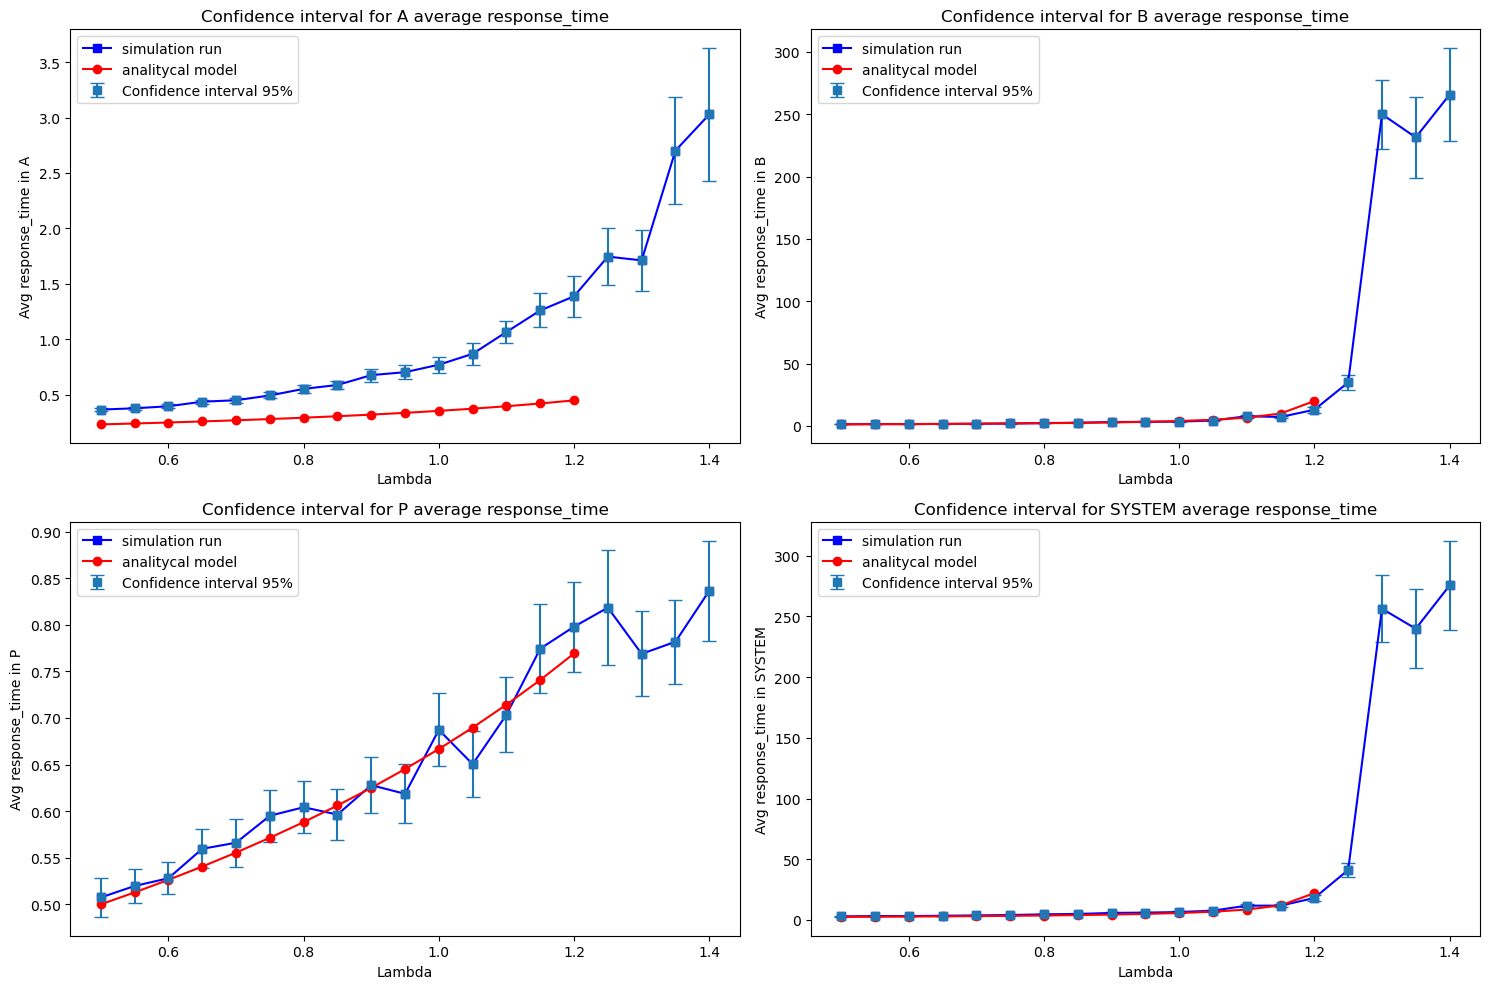
\includegraphics[width=0.75\linewidth]{figs/results/obj3/verification/obj3_lineplot_rtime.png}
    \caption{ Confronto tra valori medi della simulazione e del modello analitico dell Tempo di Risposta per l’Obiettivo 3.}
    \label{fig:enter-label}
\end{figure}   
\end{frame}